\documentclass{mcmthesis}
\mcmsetup{CTeX = false,    % 使用 CTeX 套装时,设置为 true
          tcn = {2515374}, problem = \textcolor{red}{C},
          sheet = true, titleinsheet = true, keywordsinsheet = true,
          titlepage = false, abstract = false}

\usepackage{newtxtext}     % \usepackage{palatino}
\usepackage[backend=bibtex]{biblatex}   % for RStudio Complie
\addbibresource{citation.bib}

\usepackage{tocloft}
\setlength{\cftbeforesecskip}{6pt}
\renewcommand{\contentsname}{\hspace*{\fill}\Large\bfseries Contents \hspace*{\fill}}

\title{A Good Title}

\begin{document}
       
\begin{abstract}
    
    The Olympic Games, inspired by the ancient Greek Games, is the world's premier international multi-sport event. Held every four years, it features summer and winter editions, bringing together athletes from around the globe to compete in a wide range of sports.
    For every sports lover, the Stimulation of Olympic Medals is a very interesting topic, while it's crucial for countries to adjust their strategy. 
    \textbf{In this paper, we will analyze the data of the Summer Olympic Games from 1896 to 2024, and use the data to simulate the results of the 2028 and 2032 Olympics using different methods from `PRE' model mostly based on machine learning.}

    First, we've examined, cleaned and transformed the raw data, setting the ice sports aside, combining various teams of one country, and mapped the countries which no longer exist to the current existing country.
    Then, we turn to machine learning, select the independent variables to use by \textbf{Correlation Coefficient Matrix} and \textbf{Principal Component Analysis}, split the data into training and testing parts, and use \textbf{eXtreme Gradient Boosting} methods to train features and target matrix. \textbf{Kolmogorov-Smirnov Test} is used to ensure the effectiveness of the model, while history data are reprocessed using feature importance and data in recent years are given higher weights to improve the accuracy of the model. In the end, we use the model to predict the results of the 2028 and 2032 Olympics, and the results are shown in multiple forms.

    After that, we encode country labels, create feature dataset of each country,and filter out data for countries that won medals in 1896 to construct training and testing datasets of the feature of `First Win Country'.\textbf{Random Forest} is used to train the model, and the results of the top ten countries most likely to win their first medal in 2028 are shown in the form of a bar chart.

    By analyzing the data given, we find that some specific sports and events play a significant role in the medal tally of some specific countries, e.g: long distance race for Kenya. We calculate the \textbf{proportion} of medals from these events, further estimate their importance, and finally come to the result of the extent to which choosing these events impact countries performance in the medal list.

    Finally, we combined methods used above and created a comprehensive prediction model called \textbf{`PRE'} model, naming after the primary methods we use. The model is specifically-tuned to calculate \textbf{Legendary Index} so as to detect \textbf{Great Couch Effect }using data of US gymnastics team coached by Bela Karolyi and Marta Karolyi. Lang Ping is successfully detected as a legendary coach, and we've found many more great teams and athletes, even controversial results(2024 Male Fencing,Italy) and decline of the great ranks(2024 Tennis,China).

    \textbf{Greatness is not born, but made.}We hope that our model may help countries' Olympic committes to accommodate strategies and achieve better results in the future Olympic Games.

    \begin{keywords}
    Olympic Games; Data Analysis; Stimulation; Machine Learning
    \end{keywords}
    
    \end{abstract}
    

\maketitle
\tableofcontents 
\thispagestyle{empty}   
\newpage

\section{Introduction}

\subsection{Background and Literature Review}

The Olympic Games, often simply referred to as the Olympics, are the world's foremost international multi-sport events. With a history that dates back over 2,000 years to ancient Greece, the modern Olympics were revived in 1896 by Pierre de Coubertin.
The Olympics are held every four years, with the Summer Olympics and the Winter Olympics alternating every two years. The Summer Olympics feature a vast array of sports, from athletics and swimming, which are considered the cornerstones of the Games, to more specialized sports like fencing, badminton, and gymnastics. Athletes from around the globe gather to compete at the highest level, showcasing their extraordinary skills, determination, and physical prowess.

Over the years, the Olympics have become a platform for athletes to break records, inspire generations, and promote cultural exchange. They have also had a significant impact on the host cities, driving urban development, improving infrastructure, and boosting the local economy. Despite facing various challenges, including political issues and the impact of global events, the Olympic Games continue to hold a special place in the hearts of people worldwide, symbolizing the power of sports to unite and uplift humanity.

The prediction of Olympic medal counts has long been a topic of interest among sports enthusiasts, statisticians, and researchers. Understanding how to forecast the number of medals a country or athlete might win is not only a matter of curiosity but also has implications for sports management, marketing, and national pride. 

Traditional approaches are typically made closer to the start of an upcoming Olympic Games when information about the current athletes scheduled to compete becomes available. This approach allows for a more accurate assessment of a country's or athlete's medal prospects. For example, the virtual medal table forecast by Nielsen \cite{1} provides a more real-time and data-driven prediction. By incorporating current athlete performance, injuries, and recent competition results, these modern models can better capture the dynamic nature of sports.

However, these data may be concealed and intentionally modified by countries' Olympic committees, which may produce misleading predictions.

Research in this area has also explored the use of advanced statistical techniques. Machine learning algorithms, for instance, have been employed to analyze large datasets encompassing a wide range of variables related to athletes, sports, and countries. These algorithms can identify complex patterns and relationships that might not be apparent through traditional statistical methods. For example, they can consider factors such as an athlete's training regime, mental state, and even the influence of the home crowd (in the case of host countries) on their performance.

Another aspect that has received attention is the impact of external factors on medal count predictions. Global events such as the COVID-19 pandemic have disrupted sports schedules and training routines, making it more challenging to predict medal counts accurately. Research has attempted to quantify these impacts and adjust prediction models accordingly. Additionally, political and social factors, such as doping scandals and changes in sports governance, can also have a significant influence on the outcome of Olympic competitions and, thus, on medal count predictions.

In conclusion, the field of predicting Olympic medal counts has evolved significantly over the years. While historical medal counts still provide some basis for understanding trends, the focus has shifted towards more contemporary methods that utilize real-time information about current athletes. The use of advanced statistical techniques and an increased awareness of external factors have improved the accuracy of these predictions. However, there is still room for further research, particularly in refining models to account for unforeseen events and in exploring new data sources that could enhance the predictive power of these models. As the Olympics continue to evolve, so too will the methods and models used to predict the medal counts, ensuring that this remains a vibrant and relevant area of study.

\subsection{Restatement of the Problem}
Considering the background, in this paper we are required to solvye the following problems:

\textbf{Task 1:} Develop a model for medal counts for each country, both \textbf{Gold} and \textbf{Total}, and use the model to predict various countries' performance in the 2028 and 2032 Olympics. The model also include estimates of the precision and measures of how well the model performs.

\textbf{Task 2:} Develop a model for prediciton of when a country will win its \textbf{first} medal in the Olympics, and the probabililty of winning it in the coming next LA Olympics. Also, we will evaluate this model.

\textbf{Task 3:} Develop a model for estimation of the \textbf{"great coach"} effect, and further using this model to identify three countries suitable for imitating this strategy.

\textbf{Task 4:} Calculating the \textbf{"great athlete"} effect, referring to the phenomenon that some great athletes won a large number of the (Gold) medals of a certain sport or event, and sometimes his/her country's medal tally greatly depend on him/her during his/her athlete career. We will also explain how this can inform country Olympic committees.


In order to solve those problems, we will proceed as follows:

\begin{itemize}
\item {\bf Stating assumptions}. By stating our assumptions, we will narrow the focus of our approach towards the problems and provide some insight into bathtub water temperature issues.

\item {\bf Making notations}. We will give some notations which are important for us to clarify our models.

\item {\bf Presenting our model}. In order to investigate the problem deeper, we divide our model into two sub-models. One is a steady convection heat transfer sub-model in which hot water is added constantly. The other one is an unsteady convection heat transfer sub-model where hot water is added discontinuously.

\item {Defining evaluation criteria and comparing sub-models}. We define two main criteria to evaluate our model: the mean temperature of bath water and the amount of inflow water.

\item {\bf Analysis of influencing factors}. In term of the impact of different factors on our model, we take those into consideration: the shape and volume of the tub, the shape/volume/temperature of the person in the bathtub, the motions made by the person in the bathtub and adding a bubble bath additive initially.

\item {\bf Model testing and sensitivity analysis}. With the criteria defined before, we evaluate the reliability of our model and do the sensitivity analysis.

\item {\bf Further discussion}. We discuss about different ways to arrange inflow faucets. Then we improve our model to apply them in reality.

\item {\bf Evaluating the model}. We discuss about the strengths and weaknesses of our model:

\begin{itemize}
\item[1)] ... 
\item[2)] ...
\item[3)] ...
\item[4)] ...
\end{itemize}

\end{itemize}

\subsection{Our Work}

\section{Assumptions and Notations}

\subsection*{Assumptions and Justifications}

To simplify problem, make it convenient to construct simulation model and ensure it's effectiveness, following basic assumptions are made, each of which is properly justified.

\begin{itemize}
\item {\bf Data Preprocess and Country Mapping}. 

Data is cleaned and preprocessed to make it more suitable. We set the ice sports aside, combine various teams of one country, and map the countries which no longer exist to the current existing country. It's a rather difficult task since countries have changed a lot during the past century, but it's necessary to stick to the current world map.

\item {\bf Relationship between Medal counts and Historical data}. 

Most data provided is examined to be accurate and reliable, although some may not be the same as the data provided from other sources. Few of the data is examined and changed since it's too faraway from reality. Medal counts are also assumed to be related to multiple variables:years, gender, athletes and number of sports, diciplines, events,etc.

\item {\bf Countries that will possibly take part in the 2028 Olympics}. 

Countries that have taken part in 2024 Olympics will also take part in 2028 Olympics. There's no reason for them not to attend the Olympics, and it's impossible to estimate medal of new countries if they've never taken part in the Olympics using historical data. Russia is also assumed to participate in the 2028 Olympics, whether the athletes will be able to compete under the Russian flag or not, their country is called Russia. 

\item {\bf Possible Sports in 2028}. 

There's said to be five new sports in the 2028 Olympics, but we set them aside because we don't have enough data to predict the medal counts of these events. Similarly, we set aside the sports that will be removed from the Olympics in 2028, and assume that most sports are like that in 2024 or their most common appearance in history(Such as gymnastics).


\end{itemize}

Other details will be stated in the following sections when we discuss the specific models.

\subsection*{Notations}

\begin{center}
\begin{tabular}{clcl}
{\bf Symbols} & {\bf Definitions} & {\bf Symbols} & \quad {\bf Definitions} \\[0.25cm]
$N_u$ & Number of countries that have not won a medal & $a$ &  aaaaaaaaaaaaaaaaaaaaa \\[0.2cm]
$k$ & &  & \\[0.2cm]
$c_p$ & &  &  \\[0.2cm]
$\rho$ & &  &  \\[0.2cm]
\end{tabular}
\end{center}
\noindent Define the Main parameters. Other Specific notations will be listed and explained later.

\section{Data Preprocessing}
\subsection{Data Cleaning}
\begin{itemize}
    \item \textbf{Garbled Code}
\end{itemize}

\begin{figure}[h]
    \centering
    \begin{minipage}{0.8\textwidth}
        \centering
        
\includegraphics[width=\textwidth]{../figures/bad_1.png}
        \caption{bad data}
        \label{fig:bad_1}
    \end{minipage}\hfill
    \begin{minipage}{0.2\textwidth}
        \centering
        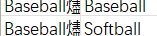
\includegraphics[width=\textwidth]{../figures/bad_2.png}
        \caption{bad text}
        \label{fig:bad_2}
    \end{minipage}
\end{figure}

We carefully examine the data and find that there are some garbled codes in the data, which may be caused by the encoding of the data. They are replaced by the correct text.

\begin{itemize}
    \item \textbf{Null, Duplicated Values and Renaming}
\end{itemize}

\begin{lstlisting}[caption=Data Cleaning]
data.fillna(0, inplace=True)
data.drop_duplicates(inplace=True)
athletes.rename(columns={'Team': 'Country'}, inplace=True)
\end{lstlisting}

Team are renamed to Country in the athletes data so that there won't be Germany-1.

\begin{itemize}
    \item \textbf{Data Splitting}
\end{itemize}

\begin{lstlisting}[caption=Data Splitting]
    data.fillna(0, inplace=True)
    data.drop_duplicates(inplace=True)
    athletes.rename(columns={'Team': 'Country'}, inplace=True)
    \end{lstlisting}

    \begin{itemize}
        \item \textbf{Remove unnecessary data}
    \end{itemize}
\begin{lstlisting}[caption=Remove Ice Sports]
    ice_sports = ['Figure Skating', 'Ice Hockey']
    programs = programs[~programs['Sport'].isin(ice_sports)]
    athletes = athletes[~athletes['Sport'].isin(ice_sports)]
\end{lstlisting}

\begin{lstlisting}[caption=Remove Program from 1906]
# Remove program from the year 1906
program = program[program['Year'] != 1906]    
\end{lstlisting}

\subsection{Country Mapping}

\begin{lstlisting}[caption=Country Mapping]
country_mapping = {# map due to the change of country in history
    'Soviet Union': 'Russia','Unified Team': 'Russia',
    'West Germany': 'Germany','East Germany': 'Germany',
    'Yugoslavia': 'Serbia',
    'Bohemia': 'Czech Republic','Czechoslovakia': 'Czech Republic',
    'Virgin Islands': 'United States',
}
# NOC mapping is similar.Only part of the country_mapping is shown here.There're also map between NOC and country.
athletes['NOC'] = athletes['NOC'].replace(noc_mapping)
medals['NOC'] = medals['NOC'].replace(country_mapping)
\end{lstlisting}

\subsection*{Primary processed data: The `Top 10s'}

\begin{figure}[h]
    \centering
    \begin{minipage}{0.4\textwidth}
        \centering
        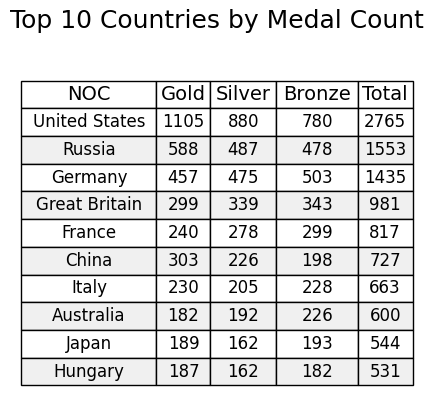
\includegraphics[width=\textwidth]{../figures/top_10_countries.png}
        \caption{top $10$ countries}
        \label{fig:top_10_countries}
    \end{minipage}\hfill
    \begin{minipage}{0.4\textwidth}
        \centering
        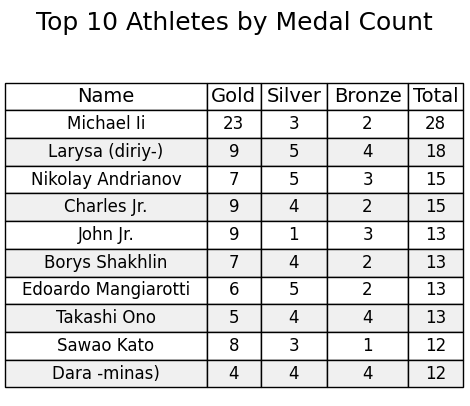
\includegraphics[width=\textwidth]{../figures/top_10_athletes.png}
        \caption{top $10$ athletes}
        \label{fig:top_10_athletes}
    \end{minipage}
\end{figure}
\section{Notations}

\begin{center}
\begin{tabular}{clc}
{\bf Symbols} & {\bf Description} & \quad {\bf Unit} \\[0.25cm]
$h$ & Convection heat transfer coefficient & \quad W/(m$^2 \cdot$ K) 
\\[0.2cm]
$k$ & Thermal conductivity & \quad W/(m $\cdot$ K) \\[0.2cm]
$c_p$ & Specific heat & \quad J/(kg $\cdot$ K) \\[0.2cm]
$\rho$ & Density & \quad kg/m$^2$ \\[0.2cm]
$\delta$ & Thickness & \quad m \\[0.2cm]
$t$ & Temperature & \quad $^\circ$C, K \\[0.2cm]
$\tau$ & Time & \quad s, min, h \\[0.2cm]
$q_m$ & Mass flow & \quad kg/s \\[0.2cm]
$\Phi$ & Heat transfer power & \quad W \\[0.2cm]
$T$ & A period of time & \quad s, min, h \\[0.2cm]
$V$ & Volume & \quad m$^3$, L \\[0.2cm]
$M,\,m$ & Mass & \quad kg \\[0.2cm]
$A$ & Aera & \quad m$^2$ \\[0.2cm]
$a,\,b,\,c$ & The size of a bathtub  & \quad m$^3$
\end{tabular}
\end{center}

\noindent where we define the main parameters while specific value of those parameters will be given later.

\section*{Model Overview}


In order to solve those problems, we will proceed as follows:

\begin{itemize}
    \begin{figure}[htbp]
        \centering
        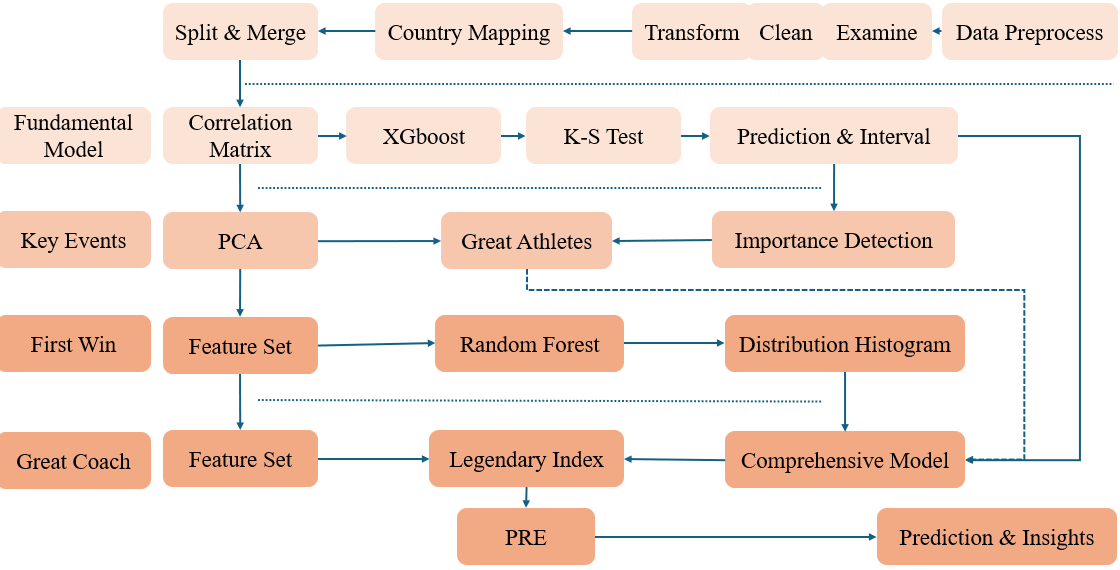
\includegraphics[width=1\textwidth]{./figures/figure1_work_flow.png}
        \caption{Flow chart}
        \label{fig:flow_chart}
    \end{figure}
    
\item {\bf Model Presentation}. We divide our task into four models: \textbf{Predicting the Medal of the 2028 LA Olympics}, \textbf{Key Events}, \textbf{Predicting First Medal Countries}, and \textbf{Great Coach Effect}.

\item {\bf Data Collection and Processing}. We gather relevant data, clean, and transform it. The data is then merged and analyzed using statistical methods to prepare it for machine learning.

\item {\bf Predictive Modeling}. We use various machine learning techniques, including \textbf{Random Forest} and \textbf{eXtreme Gradient Boosting}, to build models that predict outcomes such as the first medal countries and key events.

\item {\bf Model Validation and Analysis}. We validate our models using \textbf{KS test} and analyze the performance of athletes and countries in specific sports/events. This includes forming the \textbf{Key Event Model} and the \textbf{Great Coach Model}.

\item {\bf Results and Discussion}. We present the results of our models, discuss their implications, and provide insights into the factors influencing the outcomes of the 2028 LA Olympics.
\end{itemize}

\section{Sub-model I : Adding Water Continuously}

We first establish the sub-model based on the condition that a person add water continuously to reheat the bathing water. Then we use Computational Fluid Dynamics (CFD) to simulate the change of water temperature in the bathtub. At last, we evaluate the model with the criteria which have been defined before.

\subsection{Model Establishment}

Since we try to keep the temperature of the hot water in bathtub to be even, we have to derive the amount of inflow water and the energy dissipated by the hot water into the air.

We derive the basic convection heat transfer control equations based on the former scientists’ achievement. Then, we define the mean temperature of bath water. Afterwards, we determine two types of heat transfer: the boundary heat transfer and the evaporation heat transfer. Combining thermodynamic formulas, we derive calculating results. Via Fluent software, we get simulation results.

\subsubsection{Control Equations and Boundary Conditions}

According to thermodynamics knowledge, we recall on basic convection
heat transfer control equations in rectangular coordinate system. Those
equations show the relationship of the temperature of the bathtub water in space.

We assume the hot water in the bathtub as a cube. Then we put it into a
rectangular coordinate system. The length, width, and height of it is $a,\, b$ and $c$.

\begin{figure}[h] 
\centering
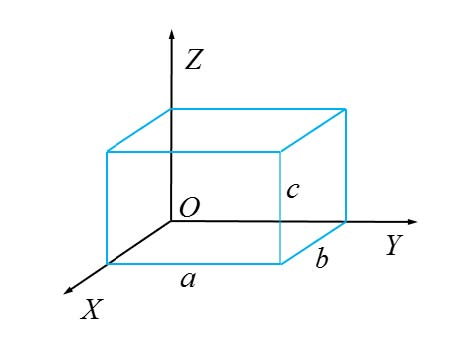
\includegraphics[width=8cm]{fig2.jpg}
\caption{Modeling process} \label{fig2}
\end{figure}

In the basis of this, we introduce the following equations \cite{5}:

\begin{itemize}
\item {\bf Continuity equation:}
\end{itemize}

\begin{equation} \label{eq1}
\frac{\partial u}{\partial x} + \frac{\partial v}{\partial y} +\frac{\partial w}{\partial z} =0
\end{equation}

\noindent where the first component is the change of fluid mass along the $X$-ray. The second component is the change of fluid mass along the $Y$-ray. And the third component is the change of fluid mass along the $Z$-ray. The sum of the change in mass along those three directions is zero.

\begin{itemize}
\item {\bf Moment differential equation (N-S equations):}
\end{itemize}

\begin{equation} \label{eq2}
\left\{
\begin{array}{l} \!\!
\rho \Big(u \dfrac{\partial u}{\partial x} + v \dfrac{\partial u}{\partial y} + w\dfrac{\partial u}{\partial z} \Big) = -\dfrac{\partial p}{\partial x} + \eta \Big(\dfrac{\partial^2 u}{\partial x^2} + \dfrac{\partial^2 u}{\partial y^2} + \dfrac{\partial^2 u}{\partial z^2} \Big) \\[0.3cm]
\rho \Big(u \dfrac{\partial v}{\partial x} + v \dfrac{\partial v}{\partial y} + w\dfrac{\partial v}{\partial z} \Big) = -\dfrac{\partial p}{\partial y} + \eta \Big(\dfrac{\partial^2 v}{\partial x^2} + \dfrac{\partial^2 v}{\partial y^2} + \dfrac{\partial^2 v}{\partial z^2} \Big) \\[0.3cm]
\rho \Big(u \dfrac{\partial w}{\partial x} + v \dfrac{\partial w}{\partial y} + w\dfrac{\partial w}{\partial z} \Big) = -g-\dfrac{\partial p}{\partial z} + \eta \Big(\dfrac{\partial^2 w}{\partial x^2} + \dfrac{\partial^2 w}{\partial y^2} + \dfrac{\partial^2 w}{\partial z^2} \Big)  
\end{array}
\right.
\end{equation}

\begin{itemize}
\item {\bf Energy differential equation:}
\end{itemize}

\begin{equation} \label{eq3}
\rho c_p \Big( u\frac{\partial t}{\partial x} + v\frac{\partial t}{\partial y} + w\frac{\partial t}{\partial z} \Big) = \lambda \Big(\frac{\partial^2 t}{\partial x^2} + \frac{\partial^2 t}{\partial y^2} + \frac{\partial^2 t}{\partial z^2} \Big)
\end{equation}

\noindent where the left three components are convection terms while the right three components are conduction terms.

By Equation \eqref{eq3}, we have ......

......

On the right surface in Fig. \ref{fig2}, the water also transfers heat firstly with bathtub inner surfaces and then the heat comes into air. The boundary condition here is ......

\subsubsection{Definition of the Mean Temperature}

......

\subsubsection{Determination of Heat Transfer Capacity}

......

\section{Sub-model II: Adding Water Discontinuously}

In order to establish the unsteady sub-model, we recall on the working principle of air conditioners. The heating performance of air conditions consist of two processes: heating and standby. After the user set a temperature, the air conditioner will begin to heat until the expected temperature is reached. Then it will go standby. When the temperature get below the expected temperature, the air conditioner begin to work again. As it works in this circle, the temperature remains the expected one.

Inspired by this, we divide the bathtub working into two processes: adding
hot water until the expected temperature is reached, then keeping this
condition for a while unless the temperature is lower than a specific value. Iterating this circle ceaselessly will ensure the temperature kept relatively stable.

\subsection{Heating Model}

\subsubsection{Control Equations and Boundary Conditions}

\subsubsection{Determination of Inflow Time and Amount}

\subsection{Standby Model}

\subsection{Results}

\quad~ We first give the value of parameters based on others’ studies. Then we get the calculation results and simulating results via those data.

\subsubsection{Determination of Parameters}

After establishing the model, we have to determine the value of some
important parameters.

As scholar Beum Kim points out, the optimal temperature for bath is
between 41 and 45$^\circ$C [1]. Meanwhile, according to Shimodozono's study, 41$^\circ$C warm water bath is the perfect choice for individual health [2]. So it is reasonable for us to focus on $41^\circ$C $\sim 45^\circ$C. Because adding hot water continuously is a steady process, so the mean temperature of bath water is supposed to be constant. We value the temperature of inflow and outflow water with the maximum and minimum temperature respectively.

The values of all parameters needed are shown as follows:

.....

\subsubsection{Calculating Results}

Putting the above value of parameters into the equations we derived before, we can get the some data as follows:

%%普通表格
\begin{table}[h]  %h表示固定在当前位置
\centering        %设置居中
\caption{The calculating results}  %表标题
\vspace{0.15cm}
\label{tab2}                       %设置表的引用标签
\begin{tabular}{|c|c|c|}  %3个c表示3列, |可选, 表示绘制各列间的竖线
\hline                    %画横线
Variables & Values & Unit     \\ \hline  %各列间用&隔开
$A_1$     & 1.05   &   $m^2$  \\ \hline
$A_2$     & 2.24   &   $m^2$  \\ \hline
$\Phi_1$  & 189.00 &   $W$   \\ \hline
$\Phi_2$  & 43.47  &   $W$   \\ \hline
$\Phi$    & 232.47 &   $W$   \\ \hline
$q_m$     & 0.014  &   $g/s$ \\ \hline
\end{tabular}
\end{table}

From Table \ref{tab2}, ......

......

\section{Correction and Contrast of Sub-Models}

After establishing two basic sub-models, we have to correct them in consideration of evaporation heat transfer. Then we define two evaluation criteria to compare the two sub-models in order to determine the optimal bath strategy.

\subsection{Correction with Evaporation Heat Transfer}

Someone may confuse about the above results: why the mass flow in the first sub-model is so small? Why the standby time is so long? Actually, the above two sub-models are based on ideal conditions without consideration of the change of boundary conditions, the motions made by the person in bathtub and the evaporation of bath water, etc. The influence of personal motions will be discussed later. Here we introducing the evaporation of bath water to correct sub-models.

\subsection{Contrast of Two Sub-Models}

Firstly we define two evaluation criteria. Then we contrast the two submodels via these two criteria. Thus we can derive the best strategy for the person in the bathtub to adopt.

\section{Model Analysis and Sensitivity Analysis}

\subsection{The Influence of Different Bathtubs}

Definitely, the difference in shape and volume of the tub affects the
convection heat transfer. Examining the relationship between them can help
people choose optimal bathtubs.

\subsubsection{Different Volumes of Bathtubs}

In reality, a cup of water will be cooled down rapidly. However, it takes quite long time for a bucket of water to become cool. That is because their volume is different and the specific heat of water is very large. So that the decrease of temperature is not obvious if the volume of water is huge. That also explains why it takes 45 min for 320 L water to be cooled by 1$^\circ$C.

In order to examine the influence of volume, we analyze our sub-models
by conducting sensitivity Analysis to them.

We assume the initial volume to be 280 L and change it by $\pm 5$\%, $\pm 8$\%, $\pm 12$\% and $\pm 15$\%. With the aid of sub-models we established before, the variation of some parameters turns out to be as follows

%%三线表
\begin{table}[h] %h表示固定在当前位置
\centering  %设置居中
\caption{Variation of some parameters}  %表标题
\label{tab7} %设置表的引用标签
\begin{tabular}{ccccccc} %7个c表示7列, c表示每列居中对齐, 还有l和r可选
\toprule  %画顶端横线
$V$      & $A_1$   & $A_2$   & $T_2$    & $q_{m1}$ & $q_{m2}$ & $\Phi_q$ \\
\midrule  %画中间横线
-15.00\% & -5.06\% & -9.31\% & -12.67\% & -2.67\%  & -14.14\% & -5.80\% \\
-12.00\% & -4.04\% & -7.43\% & -10.09\% & -2.13\%  & -11.31\% & -4.63\% \\
-8.00\%  & -2.68\% & -4.94\% & -6.68\%  & -1.41\%  & -7.54\%  & -3.07\% \\
-8.00\%  & -2.68\% & -4.94\% & -6.68\%  & -1.41\%  & -7.54\%  & -3.07\% \\
-8.00\%  & -2.68\% & -4.94\% & -6.68\%  & -1.41\%  & -7.54\%  & -3.07\% \\
-8.00\%  & -2.68\% & -4.94\% & -6.68\%  & -1.41\%  & -7.54\%  & -3.07\% \\
-8.00\%  & -2.68\% & -4.94\% & -6.68\%  & -1.41\%  & -7.54\%  & -3.07\% \\
-8.00\%  & -2.68\% & -4.94\% & -6.68\%  & -1.41\%  & -7.54\%  & -3.07\% \\
-8.00\%  & -2.68\% & -4.94\% & -6.68\%  & -1.41\%  & -7.54\%  & -3.07\% \\
-8.00\%  & -2.68\% & -4.94\% & -6.68\%  & -1.41\%  & -7.54\%  & -3.07\% \\
-8.00\%  & -2.68\% & -4.94\% & -6.68\%  & -1.41\%  & -7.54\%  & -3.07\% \\
\bottomrule  %画底部横线
\end{tabular}
\end{table}%到时候对多个问题进行分别回答,answer0只是一个模板
\section{Other Insights}

\subsection{Predict the medal of the 2032 Olympics}

\begin{figure}[h]
\centering
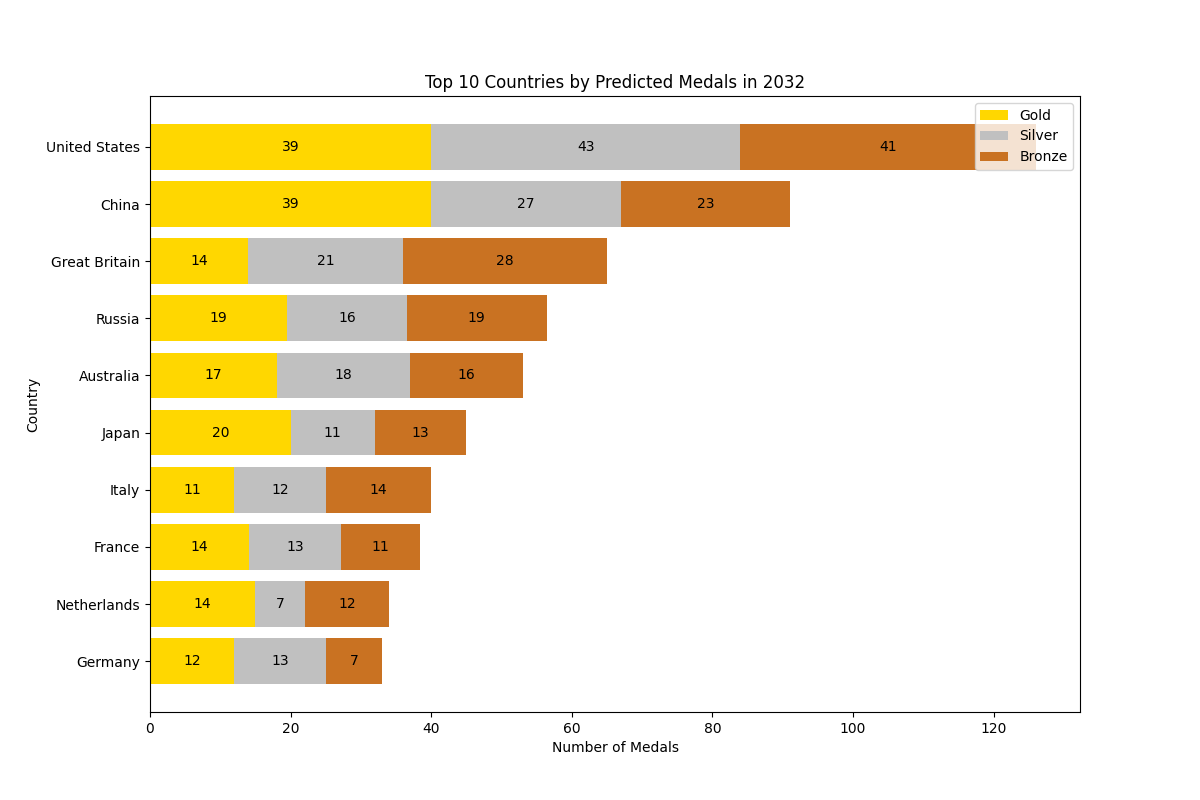
\includegraphics[width=1\textwidth]{../figures/2032.png}
\caption{Predicted Medal Counts for the 2032 Olympics}
\label{fig:medal_prediction}
\end{figure}

The prediction of 2032 Olympics is rather difficult because of the uncertainty of the future and almost no information of the 2032 Olympics. In \textbf{Figure \ref{fig:medal_prediction}}, we've tried to make some prediction with our comprehensive PRE model, taking all effects into account.Although the prediction may not be accurate enough, it can still serve as a reference.

\subsection{Greatness and the strategy of the country Olympic committees}
During the estimation of whether a country's achievement can be due to \textbf{Great Coaches}, we set a a parameter of \textbf{legendary} to evaluate the successness of a team on a certain event.
Combined with the \textbf{Great Athletes} mentioned before, we can now tell apart whether it's the great athlete(s) or the great coach that mainly contribute to great achievements.
Also, we can exclude these factors to more explicitly discuss other elements which influence various countries' performance.
\begin{figure}[h]
    \centering
    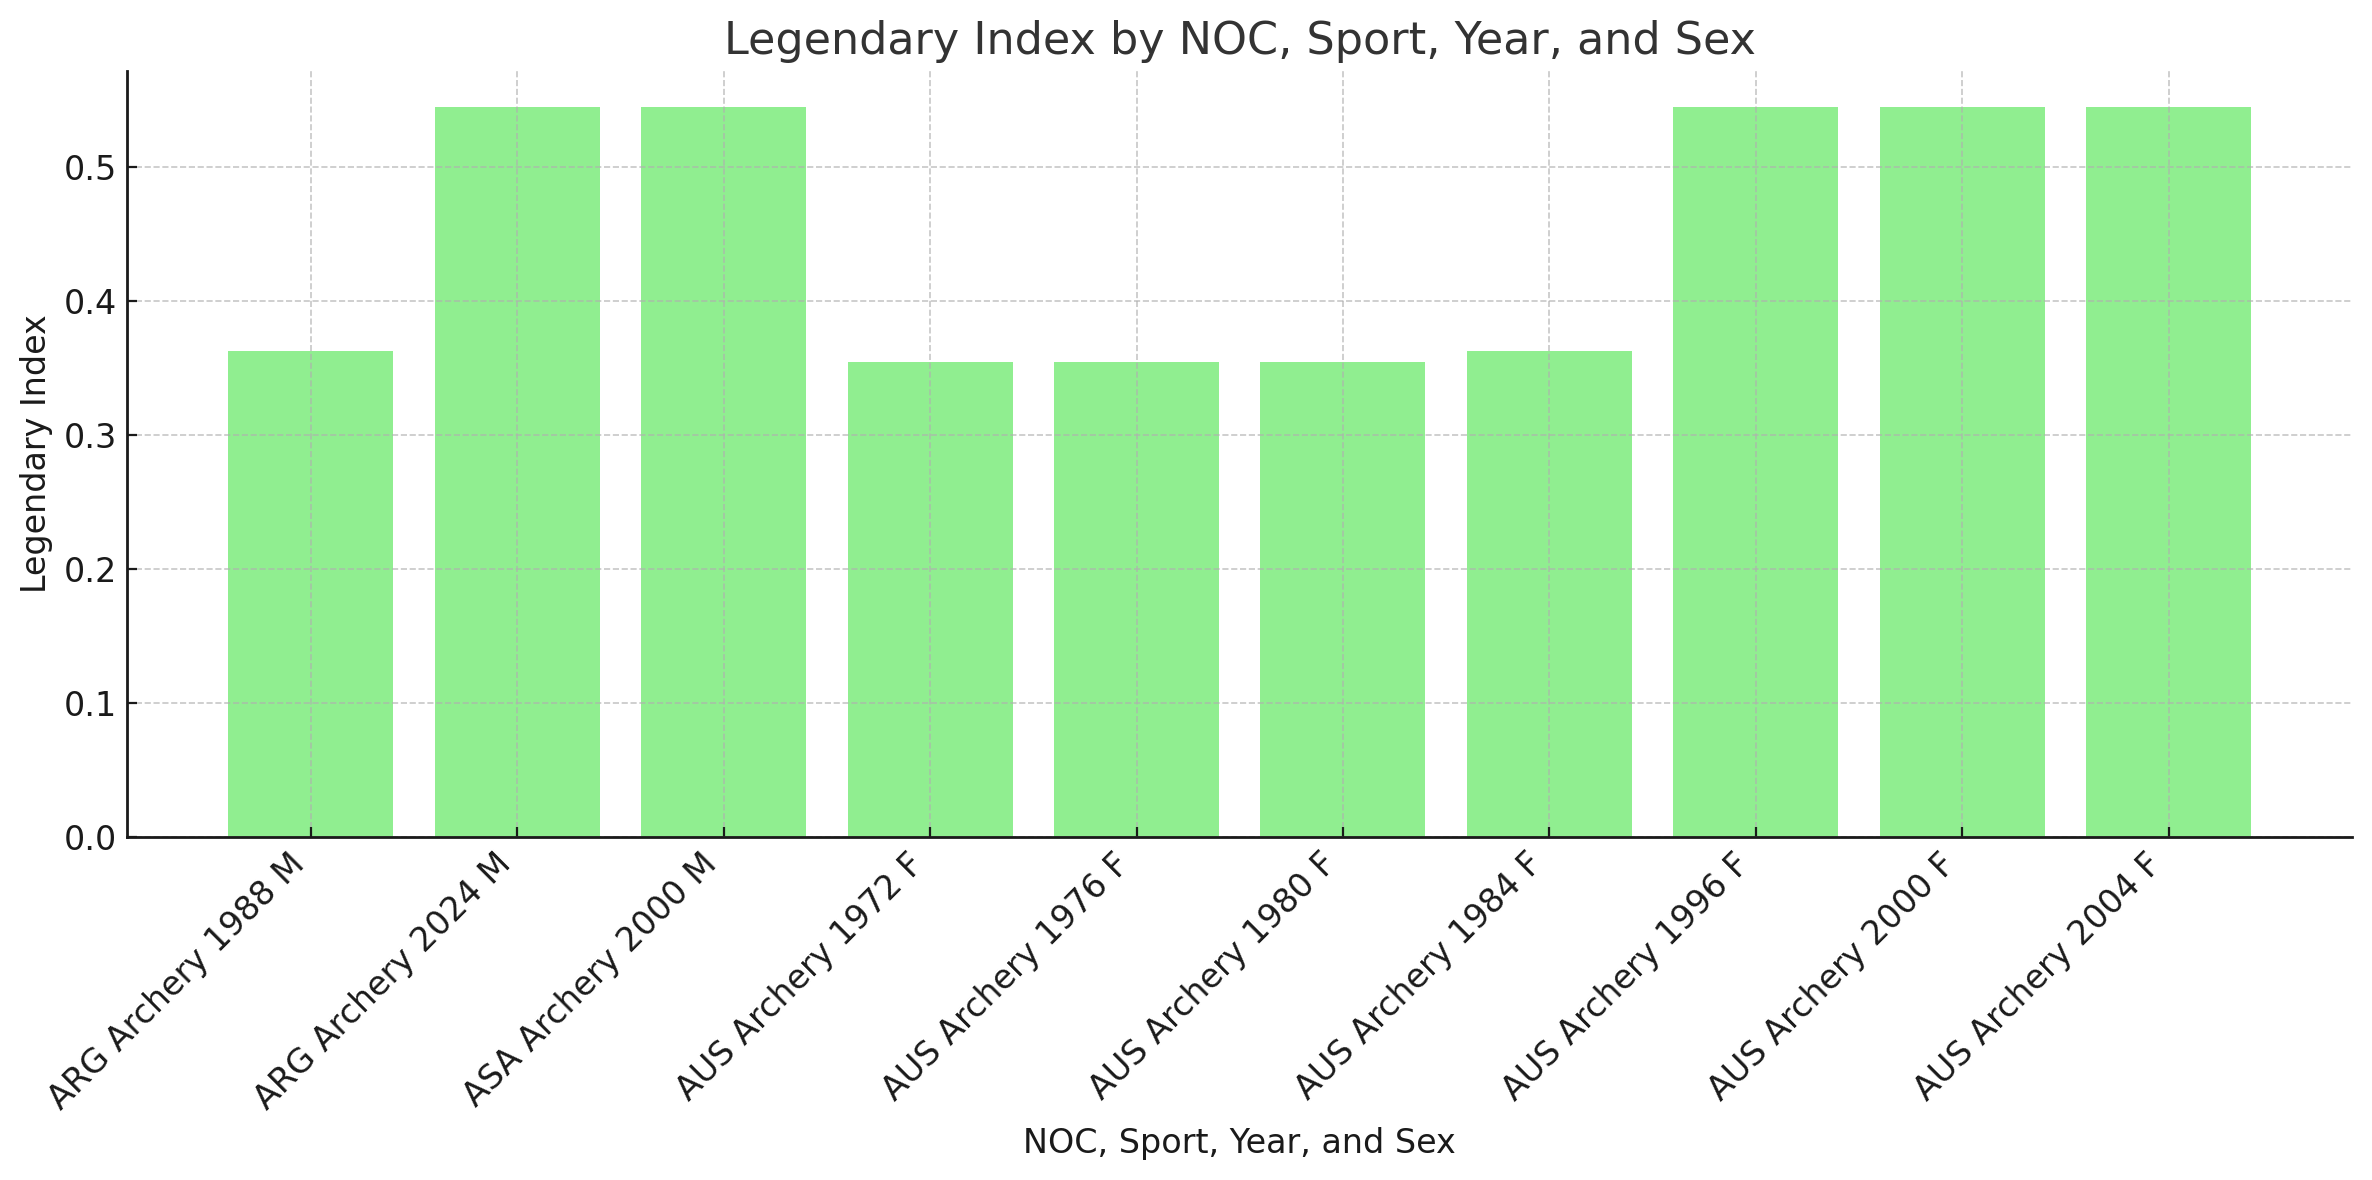
\includegraphics[width=1\textwidth]{./figures/Legendary_index.png}
    \caption{Legendary Index of certain events}
    \label{fig:legendary_index}
    \end{figure}
The graph above shows a part of the calculation result. We find out that a high \textbf{Legendary Index} is of higher probability be due to \textbf{Great Coach} when a \textbf{Great Athlete} is absent.

As to the strategy of the country Olympic committees, we give the calculation result as the suggestion that a \textbf{Legendary Index} higher than 0.68 means a high potential of future success.
It means that the committees can invest more in this certain sport/event, for example, hiring a \textbf{Great Coach} or cultivating \textbf{Great Athletes}, and hope for great achievements.\cite{jackson2014statistical}
\section{Strength and Weakness}

\subsection{Strength}

\begin{itemize}
\item We analyze the problem based on historical data with a relatively long period, so that the model we established is of great validity.

\item Our model is fairly robust due to our careful cleaning of raw data and careful selection of parameter according to real Olympic events.

\item Via Programming software, we simulate the 2028 LA Olympic results. The outcome is vivid for us to understand the prediciton.

\item We come up with testing methods to ensure precision, like KS test. Hence an overall correctness can be within reach.

\item We take multiple factors into consideration during modeling, for instance, female ratio and the continuity of participation, which add to the accuracy of our prediction model
\end{itemize}

\subsection{Weakness}

\begin{itemize}
\item We choose specific values for some peculiar parameters, for instance, we assume the proportion of female athletes of the USA team in 2028. Results may changed a bit if the female ratio is different from our assumptions.

\item Although we investigate a lot in the given data, the model is so complicated that need to be studied further with more than these data. For example, the population
of a country will impact the number of potential athletes, and further influence the country's future performance in the Olympics.

\item Limited to data amount, \textbf{Great Coach Model} is of certain sensitivity, because we can only get access to data of one or two Olympics before the great coach start tutoring.
\end{itemize}

\subsection{Further Discussions}
\subsubsection{Possible Optimization}
\begin{itemize}
    \item Due to lack of data, our model only use past data with few factors taken into account, such as year, sex and event, while neglecting other factors such as a country's population, GDP and willingness 
for medals. To be more accurate, we can add more data into our model.

    \item  Also, we can adapt more nonlinear models, besides methods like \textbf{Random Forest} , \textbf{XGBoost} , etc
    , and compare their results to be more precise on prediction.
 
    
    \end{itemize}


\subsubsection{Sensitivity Analysis : Challenges in practical application}
Although results are seemingly reasonable, there're many difficulties in practical application:

This model is potentially useful for country Olympic committees for arrangement strategies, and it only cares about data of performance, but training and taking part in the 
Olympics is a complex system, countless factors such as money investment and training period need to be considered and balanced when deciding whether to invest in a certain event or not. Since it's a complex stimulation system, our model is very sensitive to the given data. If there are more factors taken in, the results may be completely changed or may be unpredictable.

Thus, our model can only serve as a reference of prediction. There's reason why distinguished data analysis institutions always make their final forecast when the Olympics is approaching and current athletes
scheduled to compete are known : Chaos caused by Complex System is impossible to find a completely analytical solution. 
% \begin{thebibliography}{99}
%     \addcontentsline{toc}{section}{Reference}
    
%     \bibitem{1} Gi-Beum Kim. Change of the Warm Water Temperature for the Development of Smart Healthecare Bathing System. Hwahak konghak. 2006, 44(3): 270-276.
%     \bibitem{2} \url{https://en.wikipedia.org/wiki/Convective_heat_transfer#Newton.27s_law_of_cooling}
%     \bibitem{3} \url{https://en.wikipedia.org/wiki/Navier\%E2\%80\%93Stokes_equations}
%     \bibitem{4} \url{https://en.wikipedia.org/wiki/Computational_fluid_dynamics}
%     \bibitem{5} Holman J P. Heat Transfer (9th ed.), New York: McGraw-Hill, 2002. 
%     \bibitem{6} Liu Weiguo, Chen Zhaoping, ZhangYin. Matlab program design and application. Beijing: Higher education press, 2002. (In Chinese)
    
%     \end{thebibliography}
\nocite{*}
\printbibliography[title={References}]

\newpage

\begin{letter}{Enjoy Your Bath Time!}

    From simulation results of real-life situations, we find it takes a period of time for the inflow hot water to spread throughout the bathtub. During this process, the bath water continues transferring heat into air, bathtub and the person in bathtub. The difference between heat transfer capacity makes the temperature of various areas to be different. So that it is difficult to get an evenly maintained temperature throughout the bath water.
    
    In order to enjoy a comfortable bath with even temperature of bath water and without wasting too much water, we propose the following suggestions.
    
    \begin{itemize}
    \item Adding hot water consistently
    \item Using smaller bathtub if possible
    \item Decreasing motions during bath
    \item Using bubble bath additives
    \item Arranging more faucets of inflow
    \end{itemize}
    
    \vspace{\parskip}
    
    Sincerely yours,
    
    Your friends
    
    \end{letter}
    
    \newpage
    
\begin{appendices}

    \section{Code for Predicting 2028 Olympics Medal}

    \textbf{\textcolor[rgb]{0.98,0.00,0.00}{Input Python source:}}
    \lstinputlisting[language=Python]{../data_nonlinear.py}

    \section{Code for Great Coach Effect}

    \textbf{\textcolor[rgb]{0.98,0.00,0.00}{Input Python source:}}
    \lstinputlisting[language=Python]{../coach_try.py}


    \section{Code for Predicting First Medal Countries}
    
    \textbf{\textcolor[rgb]{0.98,0.00,0.00}{Input Python source:}}
    \lstinputlisting[language=Python]{../first_medal_rf.py}



    \section{Code for Great Athletes and Key Events}
    \textbf{\textcolor[rgb]{0.98,0.00,0.00}{Input Python source:}}
    \lstinputlisting[language=Python]{../key_event.py}

    
\end{appendices}
    

\newpage

\newcounter{lastpage}
\setcounter{lastpage}{\value{page}}
\thispagestyle{empty} 

\section*{Report on Use of AI}

\begin{enumerate}
\item OpenAI ChatGPT ( Dec 14, 2024 version, ChatGPT-4o ) 
\begin{description}
\item[Query1:] <insert the exact wording you input into the AI tool> 
\item[Output:] <insert the complete output from the AI tool>
\end{description}
\item Github Copilot ( 2024 version, ChatGPT-4o, o1( preview ) ) 
\begin{description}
\item[Query1:] <insert the exact wording you input into the AI tool> 
\item[Output:] <insert the complete output from the AI tool>
\end{description}

\item Deepseek ( 2025 version )
\begin{description}
    \item[Query1:] Find some references about Medal prediction in the Olympic Games 
    \item[Output:] <insert the complete output from the AI tool>
    \end{description}

\item Doubao ( 2025 version ) 
\begin{description}
\item[Query1:] The year Bela and Marta instructed the us gym team 
\item[Output:] Bela and Marta instructed the US gym team in the following years:

- \textbf{1981}: They defected to the US and began coaching gymnastics soon after.

- \textbf{1984}: They coached Mary Lou Retton, who won America's first gold medal in the Olympic all - arounds.

- \textbf{1991}: They trained Kim Zmeskal, who became the world champion.

- \textbf{1996}: Marta coached the "Magnificent Seven" member Kerri Strug to win the Olympic team gold.

- \textbf{2000}: Bela was named national team coordinator.

- \textbf{2001 - 2016}: Marta served as the coordinator of the US women's gymnastics national team.

\end{description}
\end{enumerate}


% 重置页码
\clearpage
\setcounter{page}{\value{lastpage}}

\end{document}
